\documentclass[oneside,12pt]{book}

% e-book format
\usepackage[paperwidth=210mm,paperheight=148mm,margin=10mm]{geometry}

% Cyrillization
\usepackage[T1,T2A]{fontenc}
\usepackage[utf8]{inputenc}
\usepackage[english,russian]{babel}
\usepackage{indentfirst}

% font setup for screen reading
\renewcommand{\familydefault}{\sfdefault}
\normalfont

% pdflatex options
\usepackage[unicode,colorlinks,linkcolor=blue,bookmarks=true]{hyperref}
\usepackage[pdftex]{graphicx}
\usepackage[usenames,dvipsnames,svgnames]{xcolor}

% listings
\usepackage{verbatim}
\usepackage{listings}
\lstset{
basicstyle=\small, % or \tiny \small or \footnotesize
extendedchars=true,inputencoding=utf8, % i18n
frame=single, % show frames around
numbers=left, numberstyle=\small,numbersep=1mm,% line numbering
tabsize=4, % tab style
keywordstyle=\color{Blue},%\texttt,
keywordstyle={[2]\color{Green}},%\texttt,
keywordstyle={[3]\color{Brown}},%\texttt,
keywordstyle={[4]\color{Red}},%\texttt,
keywordstyle={[5]\color{Blue}},%\texttt,
commentstyle=\color{Cyan}%\texttt%,
% showspaces=false
}

\usepackage{lstmk}\lstdefinestyle{mk}{language=mk}
\usepackage{lstrc}\lstdefinestyle{rc}{language=rc}

\newcommand{\lst}[3]{\lstinputlisting[title=\href{#2}{#1}]{#3}}
\newcommand{\lstx}[4]{\lstinputlisting[title=\href{#2}{#1},language=#4]{#3}}

% software menu & keys
\usepackage[os=win]{menukeys} 
\usepackage{amssymb} % windows key
\newcommand{\winstart}{$\boxplus$}
\newcommand{\winr}{\keys{\winstart+R}}
\newcommand{\file}[1]{\textbf{\textsf{#1}}}
\newcommand{\lms}{$\lhd$}
\newcommand{\dblms}{$\lhd\lhd$}
\newcommand{\rms}{$\rhd$}
\newcommand{\checkbox}{$\boxtimes$}
\newcommand{\uncheckbox}{$\square$}

% disable oneliner page breaks
\usepackage[defaultlines=2,all]{nowidow}

% books bib management
\usepackage{biblatex}
\addbibresource{../bib/python.bib}
\addbibresource{../bib/eskd.bib}
\addbibresource{../bib/electronics.bib}
\addbibresource{../bib/latex.bib}
\addbibresource{../bib/sat.bib}
\addbibresource{../bib/math.bib}
\addbibresource{../bib/sysdesign.bib}

\usepackage{makeidx}
\makeindex

% extra char sets
\usepackage{wasysym} % smileys

% set lists style
% \usepackage{enumitem}
% \setlist{nosep}

% misc

% \usepackage{titling}

\newcommand{\email}[1]{$<$\href{mailto:#1}{#1}$>$}
\newcommand{\internet}{Internet}

\newcommand{\cm}[1]{Cortex-M#1}
\newcommand{\cmx}{\cm{x}}

\newcommand{\linux}{Linux}
\newcommand{\emlinux}{em\linux}

\newcommand{\cpp}{$C^{+}_{+}$}
\newcommand{\py}{Python}

\newcommand{\vcs}{\hyperref[vcs]{VCS}}
\newcommand{\make}{\hyperref[make]{Make}}
\newcommand{\spice}{ngSPICE}
\newcommand{\latex}{\LaTeX}

\newcommand{\eclipse}{\textcircled{$\equiv$}\textsc{eclipse}}
\newcommand{\vim}{(g)Vim}

\newcommand{\note}[1]{\footnote{\ #1}}
\newcommand{\cp}[1]{\note{копипаста \url{#1}}}

\newcommand{\win}{\winstart Windows}

\newcommand{\mk}{МК}

\newcommand{\ram}{RAM}


\newcommand{\pref}[1]{/стр.\pageref{#1}/}

% selecting
\usepackage{framed}
\newcommand{\term}[1]{\textcolor{Green}{#1}}
\renewcommand{\emph}[1]{\textcolor{Blue}{#1}}
\newcommand{\prog}[1]{\textcolor{Brown}{#1}}
\newcommand{\pack}[1]{\textcolor{Magenta}{#1}}

% math
\usepackage{cancel}

% titles

\hypersetup{
	pdftitle={Азбука халтурщика-ARMатурщика},
	pdfauthor={ruOpenWrt, HackSpace <<Чебураторный завод>>, Консорциум хоббитов
	России, Bill Collis (Часть 1)}, 
	pdfsubject={https://github.com/ponyatov/Azbuka}
}


\author{\copyright\
\href{https://groups.google.com/forum/\#!forum/openwrt2ru}{ruOpenWrt}\\
\copyright\
HackSpace
<<\href{https://github.com/ponyatov/CHBZ/raw/master/presentation.pdf}{Чебураторный
завод}>>\\
\copyright\
Консорциум хоббитов России
}

\title{
\textbf{Азбука халтурщика-ARMатурщика}\\
разработка встраиваемых систем\\
основы бытовой автоматики,\\
систем управления и сбора данных
}

\begin{document}
\maketitle
\tableofcontents\clearpage

\clearpage\secly{О книге}

Эта книга\ --- комплект документации по аппаратно-программной платформе
ALYEH:

\begin{itemize}[nosep]
  \item \textcolor{red}{А}збука ARMатурщика
  \item \textcolor{red}{L}inux для встраиваемых систем
  \item д\textcolor{red}{Y}намический язык программирования \termdef{Ы}{Ы}
  \item библиотека \cpp\ для встраива\textcolor{red}{E}мых систем  
  \item \textcolor{red}{H}ardware библиотека универсальных модулей
\end{itemize}
\bigskip

\emph{В текущем состоянии эта книга\ --- конспект материалов, которые я сейчас
собираю, в черновой верстке. Объем материала очень большой, фактически это целая
специальность для приличного техникума, что-то типа ``Технология цифрового
производства''. Поэтому 146\% пока составляет сырая копипаста, с редкими
вкраплениями собственного бреда. В процессе адаптации, обкатки на студентах и
доработки эта поделка должна принять более вменяемый вид. Но учитывая полное
отсутствие обратной связи, этого никогда не случиться.}
\bigskip

Это учебное пособие было создано для интересующихся любительской электроникой,
самодельными цифровыми системами управления (Arduino, устройствами на
микроконтроллерах и т.п.), и программистов-лю\-би\-те\-лей. В связи с полной
деградацией системы образования пособие также рекомедуется для применения при
обучении в ВУЗах по специализациям, связанным с применением цифровой электроники
и компьютерной техники.

Большой упор был сделан на использование открытого некоммерческого программного
обеспечения, для удешевления учебного процесса, уменьшения себестоимости ваших
проектов\note{вряд ли ли у вас окажется лишняя пачка килобаксов на покупку пары
коммерческих САПР, по крайней мере пока ваш стартап не взлетит в Top\$100K}, и
стимулирования вашего участия в развитии этих программных пакетов.

Книга очень объемна и разнообразна по материалу, и построена как справочник с
группировкой материала по тематике. Для тех, кто только начинает, в разделе
\ref{learnplans}\ расписаны \termdef{пошаговые учебные планы}{учебный план} с
точки зрения параллельного изучения нескольких предметов с постепенным
усложнением\note{как это происходит при традиционном offline обучении}. Как
известно, главная часть любого обучения\ --- практическая. Особое внимание
уделено набору лабораторных работ.

\bigskip
В качестве видеоматериала были использованы 
\href{https://www.youtube.com/playlist?list=PLddc343N7YqgCWlspw08g6t0iFos9gAi4}{видеоуроки
физики}\\
\copyright\ Ерюткин Е.С., учитель физики высшей категории 
\href{http://sch1360v.mskobr.ru/}{ГБОУ СОШ №1360}, г.Москва

\bigskip
Мы признательны Bill Collis за разрешение использовать материалы его книги
<<\href{www.techideas.co.nz}{An Introduction to
Practical Electronics,
Microcontrollers and
Software Design}>> \cite{bcollis} в
русскоязычном варианте <<Азбуки>> (\ref{bcollis}), и конечно он вполне
заслуженно включен в основные соавторы этой книги.

\bigskip
Так как для работы в области электроники необходимо владение технологиями
изготовления конструктива, в книгу включен соответствующий раздел. 
Эти книги рекомендуются популярным поставщиком хоббийных настольных
микро-станков \href{http://sherline.com/}{Sherline Products}. Так как от
владельцев авторских прав не получено разрешение на полный официальный перевод,
для этих книг сделан только перевод-подстрочник, который поможет вам читать
оригинал:
\begin{itemize}
  \item Joe Martin, Craig Libuse \textbf{Tabletop Machining}
  \cite{tabletop} (\ref{tabletop})
  \item Doug Briney \textbf{Home Machinists Handbook}
  \cite{briney} (\ref{briney})
\end{itemize}

Отечественных книг по использованию маленьких ``часовых'' и настольных станков
просто не существует, хотя они и выпускались серийно. Исключение\ --- книга
Евгений Васильев \textbf{Маленькие станки} \cite{vasil}, но она имеет обзорный
характер.

\bigskip
\textbf{Лицензия на эту книгу пока не выбрана, так что она пока просто пишется в
духе OpenSource: любой может использовать ее часть, изменять или дополнять, до
тех пор, пока не накладываются какие-либо административные, финансовые или
юридические ограничения на распространение и развитие оригинальной версии или ее
открытых форков: \url{https://github.com/ponyatov/A}}
\bigskip

Приглашаем всех желающих участвовать в развитии этого учебного пособия на форум
\href{https://groups.google.com/forum/\#!forum/openwrt2ru}{ruOpenWrt} и в группу
\url{http://vk.com/samarahackerspace}, нам нужна обратная связь по качеству
материала, результаты тестирования на вас или ваших студентах, дополнения и
замечания.


\part{Основы электроники}

Здесь идет список ссылок на онлайн лекции в edX, Coursera, и т.п.

\chapter{Линейные схемы на пассивных элементах, основы электротехники}

\chapter{Симуляция и расчет схем в \spice}

\chapter{KiCAD}

\cp{http://teholabs.com/knowledge/kicad.html}

\noindent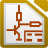
\includegraphics[height=0.5\textheight]{tmp/icon_kicad.png}


\cp{http://ru.wikibooks.org/wiki/KiCad}

KiCad\ --- распространяемый по лицензии GNU GPL программный комплекс САПР EDA с
открытыми исходными текстами, предназначенный для разработки электрических схем
и печатных плат.

Кроссплатформенность компонентов KiCad обеспечивается использованием 
библиотеки wxWidgets. Поддерживаются операционные системы Linux, 
Windows NT 5.x, Free\-BSD и Solaris.

Разработчик\ --- Жан-Пьер Шарра (фр. Jean-Pierre Charras), исследователь 
в LIS (фр. Laboratoire des Images et des Signaux\ --- Лаборатория Изображений 
и Сигналов) и преподаватель электроники и обработки изображений в фр. 
IUT de Saint Martin d’Hères (Франция).

\cp{http://ru.wikibooks.org/wiki/KiCad/Miniurok}

Этот раздел познакомит Вас с основами использования системы KiCad. Он содержит
информацию о всех шагах создания простой печатной платы: от рисования
электрической схемы до печати готового рисунка платы. Вам будут представлены
различные возможности KiCad и предложены эффективные пути решения различных
задач.

Руководство пользователя, поставляемое вместе с KiCad, содержит значительно
больше информации, чем этот урок. Ознакомтесь с ним, чтобы узнать больше об
использовании программы.



\secrel{Установка}\secdown

\secrel{\win}\label{kicadinstwin}

\menu{\winr{\url{http://www.kicad-pcb.org/}}>Download>\winstart}

\menu{\winr{\url{http://kicad.nosoftware.cz/}}>
\file{KiCad\_testing\-201x.xx.xx-BZRxxxx\_Win\_full\_version.exe}}

\bigskip

\menu{Installer Language>\emph{English}>Ok} 
в русифицированном инсталляторе кривые шрифты

\menu{KiCAD 20xx.xx.xx Setup>Next}

\menu{Лицензия>Agree}

\menu{Components>\checkbox\ все>Next}

\menu{Location>\file{C:/KiCad}>Install}

\menu{Completing Setup>\uncheckbox Wings3D>Finish}

\secrel{\linux}\label{kicadinstlin}

\begin{verbatim}
root# aptitude install kicad-doc-ru kicad
\end{verbatim}

\lst{+++\ $\sim$/.blackbox/menu}{}{/tmp/kicad.bbmenu}

\secrel{Настройка библиотек}

Для добавления библиотек, поставляемых с этой книгой, сделайте \emph{git
clone} или \emph{git pull}:

\begin{verbatim}
user:~$ git clone --depth=1 -o gh https://github.com/ponyatov/odurino.git odurino
user:~$ cd odurino
user:~/odurino$ git pull
\end{verbatim}

\menu{\prog{kicad}>\prog{eeschema}>Настройки>Библиотека}

\menu{Пользовательские пути поиска>Добавить>\file{/home/user/odurino/lib}}

\menu{Файлы библиотек>все стандартные>Удалить>OK}

\menu{Файлы библиотек>Добавить>R,L,C,SPICE,DA\_POWER,..>Открыть>OK}

\bigskip
Для проверки работы библиотек можете открыть проект

\menu{\prog{kicad}>Файл>Открыть>\file{~/Azbuka/bcollis/led1/led1.pro}}

или сразу схему

\menu{\prog{eeschema}>Файл>Открыть>\file{~/Azbuka/bcollis/led1/led1.sch}}

\secrel{Дотфайлы}

Посколько программа изначально писалась как юниксовая, пользовательские
настройки хранятся в dot-файлах:

\lst{~/.kicad}{}{kicad/kicad.dotfile}

\begin{description}
\item[KicadFrame*] размеры и положение окна менеджера проектов
\item[WorkingDir] каталог с текущим рабочим проектом
\item[fileN] список последних проектов (\ \menu{Файл>Последние файлы}\ )
\end{description}

\lst{~/.eeschema}{}{kicad/eeschema.dotfile}

\begin{description}
\item[SchematicFrame*] размеры и положение окна \prog{eeschema}
\item[fileN] список последних схем (\ \menu{Файл>Последние файлы}\ )
\end{description}

\secrel{Глобальные шаблоны}\label{kicadtemplates}

После установки \kicad\ можно скорректировать файлы глобальных шаблонов, чтобы
новые проекты создавались сразу с нужными настройками, прежде всего с нужным
нам набором библиотек:

\begin{verbatim}
sudo vim /usr/share/kicad/template/kicad.pro
\end{verbatim}

\lst{/usr/share/kicad/template/kicad.pro}{}{kicad/kicad.template}

\begin{description}
\item[LibDir] каталог библиотек, установите на свой или корпоративный/групповой
\item[LibNameN] задается список библиотек по умолчанию, приопишите ваш типовой
набор
\item[eeschema/libraries] схемные библиотеки \eeschema
\item[pcbnew/libraries] библиотеки надстеков для печатных плат \pcbnew
\end{description}

\secup


\section{Создание проекта в менеджере проектов \prog{kicad}}

В верхней части панели \term{менеджера проектов} \prog{kicad}
имеются большие кнопки запуска компонентов KiCad:

\begin{itemize}
\item \icoesch\ \prog{EeSchema}\ --- Редактор принципиальных схем
\item
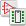
\includegraphics[height=0.1\textheight]{tmp/icon_cvpcb.png}\
\prog{CvPcb}\
--- Программа редактирования падстеков (отверстий и площадок)
\item 
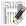
\includegraphics[height=0.1\textheight]{tmp/icon_pcbnew.png}
\prog{Pcbnew}\ ---
Редактор печатных плат
\item
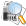
\includegraphics[height=0.1\textheight]{tmp/icon_gerbview.png}
\prog{GerbView}\ --- Программа просмотра фотошаблонов в формате Gerber
\item \prog{Bitmap2Component}\ --- Создание компонента из черно-белого
изображения (например логотипа)
\item 
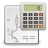
\includegraphics[height=0.1\textheight]{tmp/icon_pcbcalculator.png}
\prog{PcbCalculator}\ --- Калькулятор для печатных плат
\item 
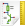
\includegraphics[height=0.1\textheight]{tmp/icon_pagelayout.png}
\prog{PageLayout}\ --- редактор формата листа схемы
\end{itemize}

Каждая кнопка запускает соответствующую программу. Мы будем использовать эти
программы по мере изучения.

\bigskip
Лучше всего для каждого проекта использовать раздельные папки; в противном
случае система может сбиться с толку, если файлы из разных проектов будут лежать
в одной папке. Проделайте следующие шаги:

\begin{enumerate}
  \item Создайте папку проекта \file{D:/ARM/SpindleDriver}
  \item Запустите программу KiCad
  \item Создайте проект (project)
  \begin{itemize}
    \item 
На панели инструментов KiCad выберите левую иконку с подсказкой\\
\menu{Начать новый проект}, используйте команду меню
\menu{Файл>Новый>Пустой} или сочетание клавиш \keys{Ctrl+N}.
    \item 
В диалоге \menu{Создать новый проект} выберите созданную папку
выберите только что созданную папку \file{D:/ARM/SpindleDriver} и
введите имя проекта \menu{\file{SpindleDriver}} и нажмите \menu{Сохранить}.
	\item
Если папка проекта содержит какие-то файлы, будет выведено окно выбора:
создать подпапку с именем проекта \menu{Yes}, или записать файл проекта
в указанную папку как есть \menu{No}. Нажмите No.
    \item 
Сохраните проект кнопкой \menu{Сохранить текущий проект}, \menu{Файл>Сохранить}
или \keys{Ctrl+S}.
	\item
В папке появится файл \file{SpindleDriver.pro}, содержащий установки вашего 
проекта. Файл имеет тектовый формат, поэтому при необходимости его можно открыть
в любом редакторе и вручную аккуратно подправить, например скорректировать
настройки зазоров печатной платы.
  \end{itemize}
\end{enumerate}

\section{Создание принципиальной схемы в \prog{eeschema}\ (часть 1)}

Запустите редактор принципиальных схем, нажав на панели KiCad большую кнопку
\icoesch.

При первом запуске \prog{eeschema}\ стартует с новым проектом и
показывает предупреждение, что файла схемы еще нет. Просто нажмите \menu{ОК}.

Если вас не устраивает черный фон рабочец области или цвета элементов схемы,
поменяйте настроки цветов \menu{Настройки>Цвета}. 

На правом краю окна редактора схем есть вертикальная панель инструментов,
которые мы и будем использовать для рисования схемы. Этими инструментами можно
выбирать объекты, размещать компоненты, вводить связи и т.д.

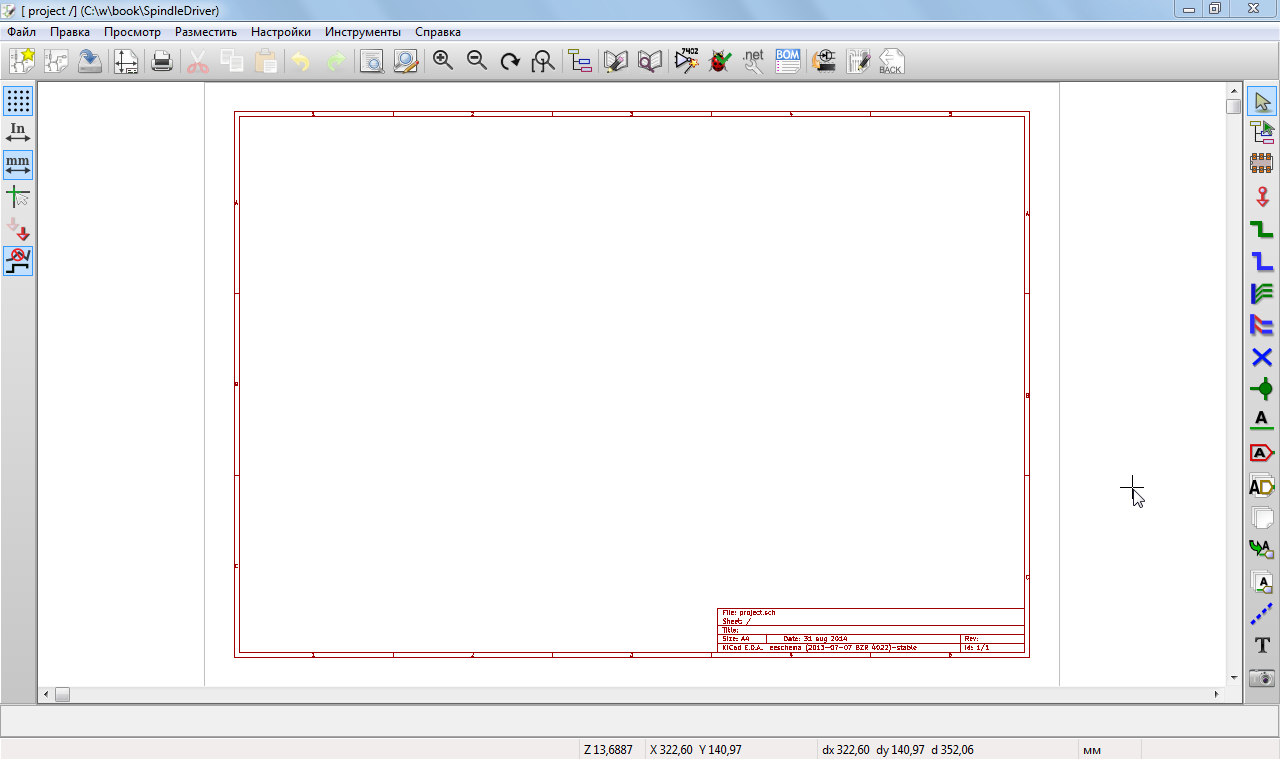
\includegraphics[width=0.9\textwidth]{kicad/ee15.png}

Завершение работы инструмента: вы можете выбрать другой инструмент из правой
инструментальной панели или же указать \menu{Отложить инструмент} по правому
клику мышки \keys{\rms}.

\section{Инструмент \emph{Добавить компоненты}}

\begin{itemize}
  \item 
На правой панели нажмите кнопку \menu{Разместить компонент}\
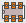
\includegraphics[height=2em]{kicad/ee21.png}. Курсор изменится со стрелки на
карандаш. Удобнее использовать сочетание клавиш \keys{Shift+A}.
Кликните в поле схемы чтобы начать размещение компонента. Появится диалог
\menu{Выбор компонента}. Вы можете выбрать компонент несколькими путями:
  \item
  \begin{enumerate}
    \item 
Если вы знаете точное имя копонента, введите его в поле \menu{Имя}, а
затем нажмите \keys{Enter} или \keys{OK}.
    \item 
Если вы знаете имя только приблизительно, в поле \menu{Имя} введите шаблон для
поиска, например, \menu{*BD*}, затем нажмите \keys{Enter} или \keys{OK}. Вы
увидите окно \\\menu{Выбрать компонент} со списком найденных компонентов.

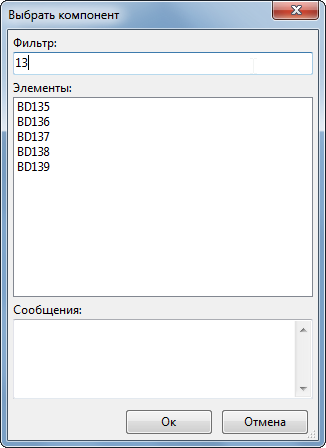
\includegraphics[height=0.5\textheight]{kicad/ee16.png}
    \item 
Вы можете искать компонент по ключевому слову, введя его в поле \menu{Имя},
затем кликнув \menu{Поиск по ключевому слову}. Однако на данный момент качество
библиотек все еще низкое, и немногие компоненты имеют ключевые слова, поэтому
эта возможность полезна косвенно.
    \item 
Можно выбрать недавно использованные компоненты из \menu{Списка истории}.
    \item 
Кнопка \menu{Список всех} вызывает диалог, в котором можно выбрать сначала
библиотеку \menu{74xx}, а затем ее компонент \menu{74HCT04}.
    \item 
Кнопка \menu{Выбор просмотром} вызывает \menu{Обзор библиотек}, позволяя
просмотреть библиотеки и находящиеся в них условные графические изображения.

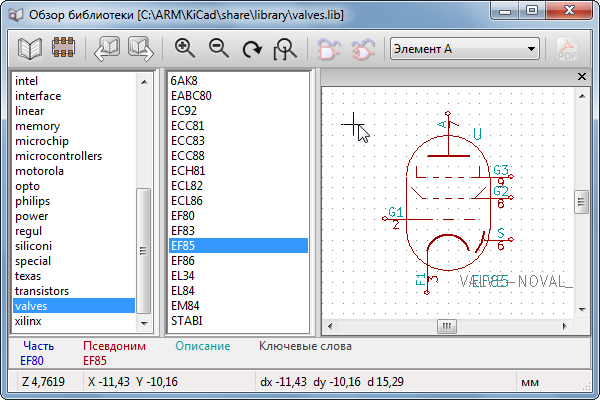
\includegraphics[height=0.5\textheight]{kicad/ee19.png}

  \end{enumerate} 
\end{itemize}

Вы также можете
вызвать обозреватель библиотек кнопкой\\
\menu{Просмотр библиотек и
компонентов}\ 
\includegraphics[height=2em]{kicad/ee20.png}

Выбрав элемент \dblms, вставьте символ в нужное место схемы \lms.
Позже вы сможете переместить его если нужно.
Зеркальное отражение компонента можно произвести следующим образом:

\begin{itemize}
  \item Поместите курсор на компоненте.
  \item По \rms\ выберите \menu{Ориентация компонента>Отражение}. 
  \item Без использования \term{контекстного меню}\ --- наведите мышь на
  компонент и нажмите кнопку \keys{X}\ или \keys{Y}.
\end{itemize}




\secrel{\prog{eeschema}: редактор электрических схем}

обеспечивает:

\begin{itemize}
\item создание однолистовых и иерархических схем,
\item проверку их корректности ERC (контроль электрических правил),
\item создание списка электрических цепей netlist для редактора топологии платы
pcbnew или для spice-моделирования схемы, 
\item доступ к документации на используемые в схеме электронные компоненты
(datasheet).
\end{itemize}


\secrel{Библиотеки компонентов}\secdown

\cp{http://habrahabr.ru/post/197582/}\bigskip

Модель компонента в САПР EDA состоит из следующих частей:

\begin{itemize}
  \item условное графическое обозначение (УГО) для схемного редактора
  \item модель компонента для редактора печатных плат (ПП)
  \item модель для симулятора (SPICE)
  \item 3D модель для передачи в универсальный САПР для работы с конструкцией
  \item дополнительные пользовательские данные: индексы компонента для
  заказа у разных поставщиков, ссылки на документацию, и т.п.
\end{itemize}

Части могут иметь несколько вариантов, например два варианта УГО (ГОСТ и ISO),
три корпуса (DIP, PLCC и LQFP), две модели для симулятора (идеальная и с
учетом паразитных эффектов), и 2 механических модели (габаритный кубик, и
подробная).

Кроме того, часто в один корпус упаковывается несколько одинаковых или разных
элементов. Одинаковые\ --- 2--4 операционных усилителя (ОУ), или вентили
логики. Разные\ --- части вакуумной лампы, разнесенные на схеме по разным
каскадам.

\bigskip

В составе KiCad поставляются библиотеки электронных компонентов (обычных и
поверхностно монтируемых SMD). Для многих библиотечных компонентов есть
3D-модели, созданные в \prog{Wings3D}.

Но как только вы начинаете работать со свежеустановленным KiCADом, тут же
обнаруживается, что библиотечные компоненты или не подходят\note{например не
соответствуют ГОСТ или стандартам предприятия}, или нужных компонентов попросту
нет в библиотеках.

Рассмотрим последовательное создание совершенно нового элемента на примере
модуля USB интерфейса HEX\_FT2232RL \ref{HEXFT2232RL}

\secrel{Создание УГО для схем}

Нам необходим встроенный редактор символов схем (библиотечных компонентов),
запускаем его следующим образом:

\begin{enumerate}
  \item Вначале запускаем \file{eeschema}
  \begin{itemize}
    \item[вверху] меню и панель инструментов
    \item[слева] область размерности и шага сетки редактора (настройка рабочей
    области)
    \item[справа] область элементов схем и перемещения по иерархии схемы
  \end{itemize}
  \item Далее запускаем встроенный
  \menu{Редактор библиотек}\ 
\includegraphics[height=2em]{kicad/ee22.png}

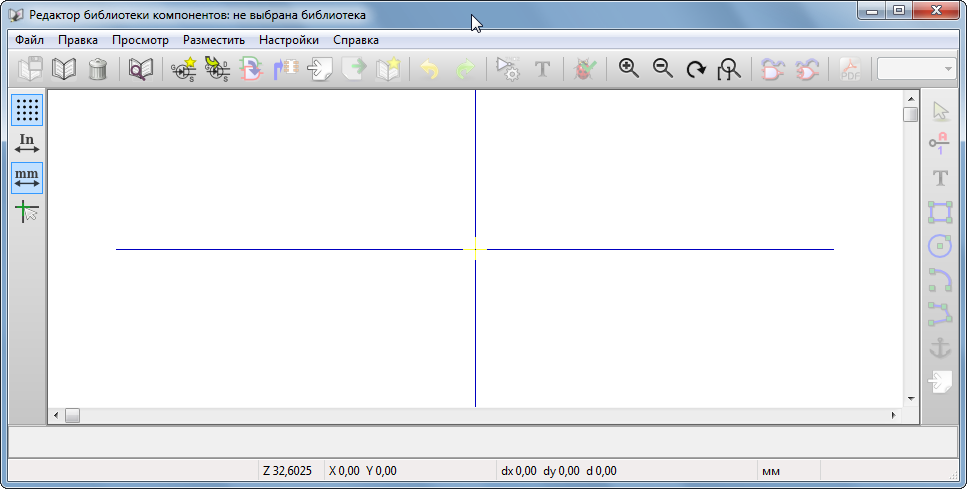
\includegraphics[height=0.5\textheight]{kicad/lib23.png}
\end{enumerate}

Необходимо создать новую библиотеку и первый собственный компонент:

\menu{Создать новый компонент}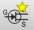
\includegraphics[height=2em]{kicad/newel.png},

\menu{Свойства компонента>Общие Настройки},

\menu{Имя компонента>HEX\_FT232RL}

\menu{Обозначение по умолчанию>U}

\menu{Количество элементов в корпусе>1}

\menu{OK}
\bigskip

В верхней панели инструментов активировались несколько кнопок, выбираем

\menu{Сохранить текущий компонент в новой библиотеке}

\includegraphics[height=2em]{kicad/lib26.png}

В открывшемся диалоге выберите каталог для библиотеки
\file{/home/user/kicad/}, и укажите имя файла (новой) библиотеки
\menu{\file{MyModules}>Сохранить}.

\bigskip
Теперь нужно добавить созданную библиотеку в рабочий список.
\bigskip

Настроим дополнительный путь, где лежат файлы библиотек. Это могут быть ваши
личные библиотеки, специальная библиотека для конкретного проекта, или комплект
библиотек поставляемых вместе с этой книгой: выберите в меню
\menu{Настройки>Библиотека}, \menu{Пользовательские пути
поиска>добавить>\file{/home/user/kicad/}}, \menu{Ok}.

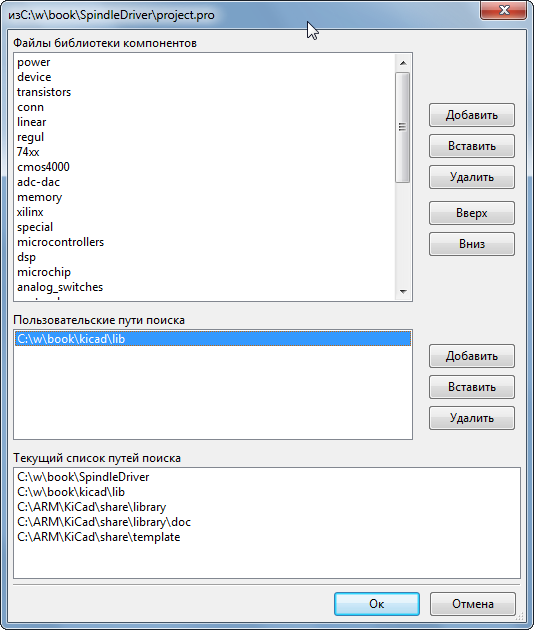
\includegraphics[height=0.5\textheight]{kicad/lib25.png}

\menu{Настройки>Библиотека},
\menu{Файлы библиотеки компонентов>power>\lms>Вставить}.
Выбираем только что созданную библиотеку \file{MyModules}.
Она будет вставлена в список до выбранной \file{power}.

\bigskip
Проделанные настройки применятся только к текущему проекту. Если Вы хотите 
чтобы новая библиотека всегда добавлялась к новым проектам, вам нужно добавить
новый путь поиска библиотек и ее название в файл шаблона, как это описано в
\ref{kicadtemplates}.

\bigskip
Если вы хотите изменить только что созданное или уже сущесствующее УГО, нужно
выбрать рабочую библиотеку, ту библиотеку в которой мы хотим работать (создавать
или редактировать компоненты). На панели инструментов нажимается кнопка

\menu{Выбор рабочей библиотеки}
\includegraphics[height=2em]{kicad/lib24.png},

\menu{Выбрать библиотеку>MyModules>Ok}.

Загружаем созданный ранее (пустой) компонент \file{HEX\_FT232RL} (или любой
другой)

\menu{Загрузить компонент для редактирования}
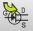
\includegraphics[height=2em]{kicad/editel.png}

\menu{Выбор компонента>Список всех>Элементы>\file{HEX\_FT232RL}>Ok}

\bigskip
\includegraphics[height=0.45\textheight]{odurino/usb/HEXFT232RL.png}

Сейчас у нас элемент не имеет графических элементов, и состоит только из
нескольких текстовых полей с обозначениями, слепленных в одной точке. Нужно их
растащить: \rms, САПР не может различить близкие элементы и уточняет для
какого поля мы хотим контекстное меню. Выбираем любое, \menu{Переместить поле}\
или кнопка \keys{M}. Перетаскиваем элемент, и \lms\ на свободном месте.

Пользуясь \ref{eskd}, отрисовываем на освободившемся месте УГО элемента,
пользуясь кнопками на панели справа. Рисование выполняется по сетке, шаг
выбирается \menu{\rms>Выбор сетки}, набор сеток фиксированный (?). При рисовании
ГОСТовских УГО округляем до ближайших дюймовых размеров\footnote{\ 1mil=1/1000
дюйма, 100mil=2.54mm=типовой шаг DIP микросхем}, или в меньшей сетке если нужно
точно гостовские размеры.

УГО имеет \term{точку привязки}, относительно которой отрисовываются элементы.
На практике важно то, что вокруг этой точки элемент вращается. Для перемещения
этой точки можно использовать кнопку

\menu{Переместить точку привязки}
\includegraphics[height=2em]{kicad/lib27.png}.

Добавляем выводы компонента: \menu{Добавить вывод
компонента}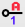
\includegraphics[height=2em]{kicad/lib28.png}.

\bigskip
Например для резистора создание выводов будет выглядеть вот так:

\bigskip
\menu{Свойства вывода}

\menu{Имя>A}

\menu{Номер>1}

\menu{Ориентация>Вправо}

\menu{Электр.тип>Пассивный}

\menu{Размер шрифта>1.27мм}

\menu{Длина>2.54мм}

\menu{Ok}

\bigskip

\menu{Имя>B}

\menu{Номер>2}

\menu{Ориентация>Влево}

\menu{Ok}

\bigskip
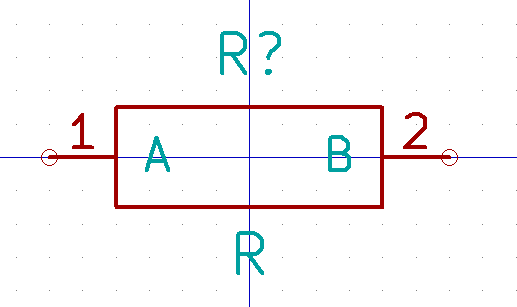
\includegraphics[height=0.5\textheight]{kicad/lib29.png}
\bigskip

Сохраняем библиотеку: \menu{Сохранить текущую
библиотеку}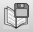
\includegraphics[height=2em]{kicad/lib30.png}

\menu{Подтверждение>Включая последние изменения компонента?>Да}

\menu{Подтверждение>Компонент существует. Изменить его?>Да}

\menu{Подтверждение>Изменить файл библиотеки ?>Да}

\secrel{Модель печатной платы}

Модель печатной платы в программе \pcbnew\ состоит из нескольких
\termdef{слоев}{слой печатной платы} с разными функциями, для типичной
двухслойной ПП:

\begin{itemize}
  \item верх
  \begin{description}
  \item[Front] медь верхнего слоя
  \item[Adhes\_Front] карта нанесения клея для компонентов
  \item[SoldP\_] карта нанесения паяльной пасты
  \item[SilkS\_] шелкография: маркировка элементов, надписи, и т.п.
  \item[Mask\_] паяльная маска 
  \end{description}
  \item низ
  \begin{description}
  \item[Back] медь нижнего слоя
  \item[Adhes\_Back] карта нанесения клея для компонентов 
  \end{description}
  \item контуры
  \begin{description}
  \item[Контур ПП] слой определяющий физ.геометрию платы, используется при
  фрезеровке контуров, сверлении монтажных отверстий, разделке сверловкой и т.п.
  \item[Пояснения] вспомогательная текстовая информация
  \item[Чертеж] вспомогательная графическая информация: габаритные размеры, зоны
  монтажа,..
  \end{description}

\item В зависимости от технологии производства и пожеланий разработчика могут
добавляться любые дополнительные слои.
\end{itemize}

\secrel{Создание падстека}

\termdef{Падстек}{падстек}\ --- модель контактной площадки компонента, в виде
набора геометрий отдельно для каждого \term{слоя} печатной платы. Также включает
информацию о диаметре сверления.

% \secrel{PS:}
% 
% Компоненты и посадочные места корпусов можно ассоциировать с документацией,
% ключевыми словами и осуществлять быстрый поиск компонента по функциональному
% назначению.
% 
% \secup
% 
% \secru{Отрисовка схемы (часть 2)}
% 
% \secdown
% 
% \secru{Автоматическое обозначение элементов}
% 
% Автоматическое обозначение элементов и перенумерация выполняется кнопкой\\
% \menu{Обозначить компоненты на
% схеме}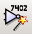
\includegraphics[height=2em]{kicad/ee000004.png}
% 
% \secru{Генерация списка цепей}
% 
% Список цепей (нетлист) используется для передачи информации о соединении
% компонентов между программами. Чаще всего СЦ создается после отрисовки схемы для
% передачи данных в программу трассировки печатной платы (ПП).

\secup


\secrel{\prog{gerbview}: просмотр фотошаблонов}

позволяет просматривать Gerber-файлы перед передачей печатных плат в
производство.


\section{Программа \prog{Wings3D} для создания 3D моделей}

Эта программа может вам пригодиться если вы планируете создавать 3D модели для PCB элементов.

Архив и файлы документации (Linux и Windows) в папке kicad/wings3d.

Взгляните на домашнюю страницу Wings3D чтобы узнать подробнее о программе.

pcbnew использует файлы в формате wrml (.wrl) экспортируемые из Wings3D (родной формат Wings3D - это .wings).

\subsection{Установка \prog{Wings3D} под \win}

\menu{\winr{\url{http://www.wings3d.com/}}>Downloads>Stable Release>\win
(32/64b)}

\menu{file{wings-n.n.n.exe}}

\menu{Compononets>\checkbox QuickLaunch>Next}

\menu{Location>\file{C:/Program Files/wings3d\_n.n.n}>Next>Install>Close}% 



\chapter{Простейшие полупроводниковые элементы}

\section{Оптоэлектроника}

\section{Схемы на биполярных транзисорах} 

\section{Схемы на на полевых транзисорах}

\chapter{Операционные усилители}

\chapter{Источники питания}

\section{Батарейное питание}

\section{Линейные стабилизаторы}

\section{Импульсные преобразователи на ШИМ-контроллерах} 

\section{Цепи защиты и гашения кондуктивных помех}

\chapter{Цифровая электроника}

\chapter{Компьютерные интерфейсы}

\section{Поколение 90х: COM, LPT, ISA}

\subsection{Резервный программатор AVR ``пять проводков''}

\section{Сеть CAN}

\section{Интерфейсные модули USB}

\subsection{Универсальный высокоскоростной конвертер FTDI FT2232H}

\subsection{JTAG-адаптер}

\subsection{Отладочный модуль CAN}

\section{Интерфейсные модули Ethernet}

\chapter{ПЛИС}

\chapter{Датчики}

\chapter{Электропривод и исполнительные устройства}

\part{Основы конструирования РЭС}

\chapter{Пакеты моделирования на основе OpenFOAM}

\chapter{Обеспечение теплового режима}

\chapter{Электромагнитная совместимость}

\section{Кондуктивные помехи}

\section{Компоновочные модели и оптимизация кабельной сети}

\part{Технология РЭС}

\chapter{Трассировка плат и подготовка производства в KiCAD}

\section{Технология ЛУТ (Лазерный УТюг)}

\section{Технология фоторезиста}

\section{Формат Gerber и подготвка промышленного производства}

\chapter{FreeCAD}

\section{Чертеж}

\section{Эскиз}

\section{Деталь}

\section{Сборка}

\section{Автогенерация конструкторской докуметации}

\section{Скрипты и пользовательские расширения}

\chapter{Эксплуатация станочного оборудования}

\chapter{Основы ЧПУ и цифрового производства}

\section{CAM-пакеты для FreeCAD}

\part{Основы теории систем автоматического управления}

\chapter{Математический аппарат}

\section{Передаточная функция}

\section{Устойчивость САУ}

\section{Сети Петри}

\section{Автоматы Маркова}

\chapter{Релейное управление}

\chapter{Пропорциональные САУ}

\chapter{ПИДn-регуляторы}

\part{Разработка ПО для встраиваемых систем}

\chapter{Вспомогательные скрипты на языке Python}

\chapter{Make: управление сборкой проектов}

\chapter{VCS: cистемы контроля версий}

\section{CVS}

\section{Subversion}

\section{Git}

\subsection{GitHub}

\chapter{Основы Си и \cpp}

\subsection{Установка MinGW (win32)}

\section{Особенности \cpp\ в embedded}

\chapter{LLVM и разработка собственных компиляторов}

\section{Лексический и синтаксический анализ}

\section{Применение flex/bison для разбора текстовых форматов данных}

\section{Компилятор Паскаля}

\chapter{Сборка кросс-компилятора GNU toolchain}

\part{Микроконтроллеры \cmx}

\part{Периферия}

\part{Встраиваемый \emlinux}

\chapter{cross}

\chapter{BuildRoot}

\chapter{Особенности OpenWrt}

\chapter{Библиотека SDL}

\section{Реализация microGUI}

\chapter{Приложения для X Window}

\chapter{Программирование сетевых приложений}

\chapter{Сборка кросс-компиляторя GNU мальтийским крестом}

\part{IDE \eclipse}


\part{Подготовка публикаций в \latex}

\cp{https://ru.wikipedia.org/wiki/LaTeX}

LaTeX (по-русски произносится \textbf{лат\'eх})\ --- наиболее популярный набор
макрорасширений (или макропакет) системы компьютерной вёрстки \TeX, который
облегчает набор сложных документов. В типографском наборе форматируется как
\LaTeX.

Главная идея \latex\ состоит в том, что авторы должны думать о содержании, о
том, что они пишут, не беспокоясь о конечном визуальном облике (печатный
вариант, текст на экране монитора или что-то другое). Готовя свой документ,
автор указывает логическую структуру текста (разбивая его на главы, разделы,
таблицы, изображения), а \latex\ решает вопросы его отображения. Так содержание
отделяется от оформления. Оформление при этом или определяется заранее
(стандартное), или разрабатывается для конкретного документа.

В практическом смысле использование \latex\ позволяет (в порядке уменьшения
важности):
\begin{itemize}
  \item с помощью макросов и \TeX-программирования реализовывать любые стили и
  самую сложную верстку, существует множество готовых пакетов для верстки
  графических химических формул, разнообразных схем, транскрипционных знаков,
  внезапно электронных схем, цветных листингов и т.п. 
  \item автоматизировать работу с документами: пересобирать выходные файлы через
  \make, генерировать части документов с помощью своих скриптов\note{отчеты,
  стандартные формы, результаты работы любых программ}
  \item получить выходой документ в .pdf .html .txt .PostScript .djvu \ldots с
  кликабельными ссылками, анимированными, а иногда и интерактивными элементами
  \item не использовать файлы документов в закрытом формате
  \item легко держать набор файлов в \vcs
  \item не покупать текстовый процессор
\end{itemize}

Особенно важен пункт про сложную верстку: она всегда нужна в крупных технических
публикациях, особенно в учебной литературе, или отчетных работах. Вам
обязательно понадобиться вставлять графики экспериментальных данных, тематически
специфичные схемы, листинги, выходные данные работы ваших пограмм и т.п.

Традиционно \latex\ любим математиками, и всеми кто готовит публикации с большим
количеством формул и перекрестных ссылок: после небольшого обучения формулы
вводятся с листа со скоростью набора текста, особенно если ваш редактор умеет
\hyperref[autocomplition]{автодополнение}, и никакой мышиной возьни.

Естественно всякие чисто автоматические вещи типа автонумерации ссылок и формул,
сборки оглавлений и индексов, цветовая подсветка синтаксиса в листингах
программ, размещение \hyperref[floatfig]{плавающих иллюстраций} и т.п.
выполняются автоматически \TeX-процессором в пакетном режиме, и на выходе
получается красивый печатный или электронный (.pdf) документ.

Единственная область, не удобная в \latex-верстке\ --- создание сложных таблиц.
Для этого были созданы визуальные редакторы, позволяющие отрисовать структуру
таблицы мышью, а затем заполнить готовый шаблон данными.

\section{Установка MikTeX под \win}
\section{Структура документа}
\subsection{Заголовочный файл или блок}
\subsection{Стили документа}
\subsection{Пакеты}
\subsection{Автор и название}
\subsection{Верстка титульных страниц}
\subsection{Оглавление}
\section{Верстка слайдов}
\section{Список литературы и цитирование}

\latex\ умеет мощную подсистему управления цитированием и списками литературы.
В простейшем случае, например при написании единственной статьи, раздел
\term{библиографии}\ можно создать в том же документе, добавив в конец
\verb|thebibliography|:

\begin{verbatim}
\documentclass{article}

\documentclass[oneside,12pt]{book}

% e-book format
\usepackage[paperwidth=210mm,paperheight=148mm,margin=10mm]{geometry}

% Cyrillization
\usepackage[T1,T2A]{fontenc}
\usepackage[utf8]{inputenc}
\usepackage[english,russian]{babel}
\usepackage{indentfirst}

% font setup for screen reading
\renewcommand{\familydefault}{\sfdefault}
\normalfont

% pdflatex options
\usepackage[unicode,colorlinks,linkcolor=blue,bookmarks=true]{hyperref}
\usepackage[pdftex]{graphicx}
\usepackage[usenames,dvipsnames,svgnames]{xcolor}

% listings
\usepackage{verbatim}
\usepackage{listings}
\lstset{
basicstyle=\small, % or \tiny \small or \footnotesize
extendedchars=true,inputencoding=utf8, % i18n
frame=single, % show frames around
numbers=left, numberstyle=\small,numbersep=1mm,% line numbering
tabsize=4, % tab style
keywordstyle=\color{Blue},%\texttt,
keywordstyle={[2]\color{Green}},%\texttt,
keywordstyle={[3]\color{Brown}},%\texttt,
keywordstyle={[4]\color{Red}},%\texttt,
keywordstyle={[5]\color{Blue}},%\texttt,
commentstyle=\color{Cyan}%\texttt%,
% showspaces=false
}

\usepackage{lstmk}\lstdefinestyle{mk}{language=mk}
\usepackage{lstrc}\lstdefinestyle{rc}{language=rc}

\newcommand{\lst}[3]{\lstinputlisting[title=\href{#2}{#1}]{#3}}
\newcommand{\lstx}[4]{\lstinputlisting[title=\href{#2}{#1},language=#4]{#3}}

% software menu & keys
\usepackage[os=win]{menukeys} 
\usepackage{amssymb} % windows key
\newcommand{\winstart}{$\boxplus$}
\newcommand{\winr}{\keys{\winstart+R}}
\newcommand{\file}[1]{\textbf{\textsf{#1}}}
\newcommand{\lms}{$\lhd$}
\newcommand{\dblms}{$\lhd\lhd$}
\newcommand{\rms}{$\rhd$}
\newcommand{\checkbox}{$\boxtimes$}
\newcommand{\uncheckbox}{$\square$}

% disable oneliner page breaks
\usepackage[defaultlines=2,all]{nowidow}

% books bib management
\usepackage{biblatex}
\addbibresource{../bib/python.bib}
\addbibresource{../bib/eskd.bib}
\addbibresource{../bib/electronics.bib}
\addbibresource{../bib/latex.bib}
\addbibresource{../bib/sat.bib}
\addbibresource{../bib/math.bib}
\addbibresource{../bib/sysdesign.bib}

\usepackage{makeidx}
\makeindex

% extra char sets
\usepackage{wasysym} % smileys

% set lists style
% \usepackage{enumitem}
% \setlist{nosep}

% misc

% \usepackage{titling}

\newcommand{\email}[1]{$<$\href{mailto:#1}{#1}$>$}
\newcommand{\internet}{Internet}

\newcommand{\cm}[1]{Cortex-M#1}
\newcommand{\cmx}{\cm{x}}

\newcommand{\linux}{Linux}
\newcommand{\emlinux}{em\linux}

\newcommand{\cpp}{$C^{+}_{+}$}
\newcommand{\py}{Python}

\newcommand{\vcs}{\hyperref[vcs]{VCS}}
\newcommand{\make}{\hyperref[make]{Make}}
\newcommand{\spice}{ngSPICE}
\newcommand{\latex}{\LaTeX}

\newcommand{\eclipse}{\textcircled{$\equiv$}\textsc{eclipse}}
\newcommand{\vim}{(g)Vim}

\newcommand{\note}[1]{\footnote{\ #1}}
\newcommand{\cp}[1]{\note{копипаста \url{#1}}}

\newcommand{\win}{\winstart Windows}

\newcommand{\mk}{МК}

\newcommand{\ram}{RAM}


\newcommand{\pref}[1]{/стр.\pageref{#1}/}

% selecting
\usepackage{framed}
\newcommand{\term}[1]{\textcolor{Green}{#1}}
\renewcommand{\emph}[1]{\textcolor{Blue}{#1}}
\newcommand{\prog}[1]{\textcolor{Brown}{#1}}
\newcommand{\pack}[1]{\textcolor{Magenta}{#1}}

% math
\usepackage{cancel}

% titles

\hypersetup{
	pdftitle={Азбука халтурщика-ARMатурщика},
	pdfauthor={ruOpenWrt, HackSpace <<Чебураторный завод>>, Консорциум хоббитов
	России, Bill Collis (Часть 1)}, 
	pdfsubject={https://github.com/ponyatov/Azbuka}
}


\author{Вася Пупкин}
\title{Пример статьи с цитатами}

\begin{document}
\maketitle
	
В статье используются книги: \cite{A} и \cite{B}
	
\begin{thebibliography}{99}

\bibitem{A} Книга А

\bibitem{B} Книга B
	
\end{thebibliography}
\end{document}
\end{verbatim}

Но если вы регулярно работаете с документацией, или часто пишете статьи,
возникает естественное желание вынести весь список литературы в отдельную базу
данных, прописать авторов, названия, издательства и т.п. Это делается с помощью
программы \file{biber}\ и пакета \file{biblatex}.

Пример использования этой системы вы легко найдете в исходниках этой книги:

\begin{itemize}
  \item файл \file{header.tex} содержит секцию подключения пакета и подгрузки
  библиофайлов:
  \begin{verbatim}% books bib management
\usepackage{biblatex}
\addbibresource{../bib/python.bib}
\addbibresource{../bib/eskd.bib}
...\end{verbatim}
  \item библиофайлы хранятся в \textbf{соседнем}\ репозитории \file{../bib},
  склонированном с \url{https://github.com/ponyatov/bib}.
  \item порядок вызова \file{pdflatex}\ и \file{biber}\ см. \file{Makefile}
\end{itemize}

Для оформления библиографии в нужном стиле см. примеры \cite{bibiso}.

\section{Команды секционирования: часть, глава, раздел,..}
\section{Таблицы}
\section{Формулы}
\section{Перекрестные ссылки и гипессылки}
\section{Листинги скриптов и текстовых данных}
\section{Подготовка иллюстраций}

Подготовка иллюстраций\ --- одна из самых геморных тех в создании документации,
и ее верстке для бумажных и электронных изданий.

Предпочтение нужно отдавать векторным форматам, за исключеним фотоиллюстраций.
В идеале скриншоты также хорошо бы переводить в векторыный формат, но пока
инструмент для этого не найден, поэтому выходные файлы будут пухнуть в объеме.

Для подготовки векторных иллюстраций: схем, графиков, диаграмм и т.п.
используйте пакеты, принимающие на вход программы на специализированном языке
программрования, легко читаемым человеком. В этом случае у вас сохраниться
отслеживать изменения, читая логи \vcs.

Обратите внимание на возможность использования стилевых файлов на весь проект
(для всех иллюстраций в книге например). Их использование даст профессиональный
вид продукту, при этом сохраниться возможность взять и переформатировать 100500
схем в 10-томнике, поменяв шрифт, цвета, толщины линий, зазоры между элементами
и т.п. 

Пользуйтесь только относительными единицами размеров, и привязывайтесь к
размерам шрифтов, это даст возможность использовать готовую иллюстрацию в
нескольких проектах с разными размерами бумаги и наборами используемых шрифтов.

\subsection{Графики GNUPLOT}

Самый постой способ получит график простой аналитической функции или
экспериментальных данных\ --- воcпользоваться утилитой
\href{http://gnuplot.info/}{GNUPLOT}.

\bigskip
Оценить возможности можно вот по этому
\href{http://upload.wikimedia.org/wikipedia/commons/b/b2/Gnuplot.ogv}{видео}

\bigskip
Примеры
\href{http://commons.wikimedia.org/wiki/Category:Gnuplot\_diagrams}{на
википедии}

\bigskip
Примеры выложенные вместе с текстом
\href{http://commons.wikimedia.org/wiki/Category:Images\_with\_Gnuplot\_source\_code}{на
языке gnuplotа}

\subsection{Схемы и графы в GraphViz}

Для отрисовки графов и схем, легко к ним сводящихся, можно использовать пакет
\file{GraphViz}\ и язык \file{Dot}. 

\subsection{PGF/TikZ}

Сложные графики можно рисовать с помощью пакета \file{PGF/TikZ}, но для его
работы нужна установленная \latex-система. Этот пакет предназначен прежде всего
для набора и верстки изданий с множеством сложных схем.

\subsection{GLE}

GLE\ --- универсальный язык описания векторных графических объектов с
элементами языка программирования. Поддерживает вычисления, типовые конструкции
программирования (циклы, условия, рекурсию).

\begin{itemize}
  \item\href{http://glx.sourceforge.net/examples/2dplots/index.html}{графики}
  \item\href{http://glx.sourceforge.net/examples/3dplots/index.html}{3D графики}
  \item\href{http://glx.sourceforge.net/examples/diagrams/index.html}{диаграммы}
  \item\href{http://glx.sourceforge.net/examples/fractals/index.html}{фракталы}
  \item\href{http://glx.sourceforge.net/examples/electronic/index.html}{электронные
  схемы}
  \item\href{http://glx.sourceforge.net/examples/other/index.html}{исчо}
\end{itemize}



\end{document}
